%% Bioinformatics Application Note
%% ---------------------------------------------------------------------------
%% Built on the article class with the two-column, 86 mm layout the journal's
%% author guidelines specify for TeX submissions. It needs no journal class
%% file and compiles on a minimal TeX installation, which is why it is the
%% default here.
%%
%% To use the official OUP class instead, see README.md. Only the front matter
%% below is class-specific; sections.tex and stats.tex are not. Supplementary
%% Table S1 lives in supplementary.tex, compiled separately.
%% ---------------------------------------------------------------------------

\documentclass[twocolumn,10pt,a4paper]{article}

% --- page geometry: two 86 mm columns ---------------------------------------
\usepackage[a4paper,textwidth=178mm,textheight=248mm,centering]{geometry}
\setlength{\columnsep}{6mm}

% --- packages ---------------------------------------------------------------
% Only packages present in a minimal TeX Live install are required. Times is
% used where available, as it is on Overleaf.
\usepackage[T1]{fontenc}
\usepackage[utf8]{inputenc}
\IfFileExists{times.sty}{\usepackage{times}}{}
\usepackage{graphicx}
\usepackage{booktabs}
\usepackage{amsmath}
\usepackage{xcolor}
\usepackage[numbers,round]{natbib}
\usepackage[colorlinks=true,allcolors=blue!60!black]{hyperref}

\bibliographystyle{plainnat}
\setcitestyle{authoryear,round}

% --- headline numbers, shared with Supplementary Table S1 (generated) -------
% Generated by scripts/make_benchmarks.py --latex -- do not edit by hand.
% Regenerate before submission so the prose matches Table 1.
\newcommand{\NumDatasets}{20}
\newcommand{\NumCells}{991,954}
\newcommand{\NumObjects}{74,037}
\newcommand{\SourceSize}{26.9}
\newcommand{\StoreSize}{8.5}
\newcommand{\MedianPfifty}{1.0}
\newcommand{\MaxPfifty}{2.4}
\newcommand{\MaxKbPerGene}{1.6}
\newcommand{\BiggestCells}{270,493}


\pagestyle{plain}

%% TODO: complete the author list and affiliations before submission.
\newcommand{\Authors}{Author One$^{1}$, Author Two$^{1}$ and
Roman Sankowski$^{1,*}$}
\newcommand{\AffilOne}{$^{1}$Affiliation, City, Country}
\newcommand{\AffilNote}{$^{*}$To whom correspondence should be addressed.}

\title{\vspace{-10mm}\bfseries A serverless browser for published single-cell
and spatial datasets}
\author{}
\date{}

\begin{document}

\twocolumn[
  \begin{@twocolumnfalse}
    \maketitle
    \vspace{-18mm}
    \begin{center}
      \Authors
      \par\vspace{4pt}
      {\small\itshape \AffilOne}
      \par\vspace{2pt}
      {\small\itshape \AffilNote}
    \end{center}
    \vspace{6mm}
    \begin{center}
    \begin{minipage}{0.88\textwidth}
      \small
      \noindent\textbf{Summary:} Single-cell datasets accompanying a publication
      are usually shared as serialised R objects that only readers with a
      matching software stack and sufficient memory can open. We present a
      pipeline that converts collections of Seurat and RaceID objects into cloud-optimised
      AnnData-Zarr stores and generates a static web viewer over them.
      Expression is stored as a dense array chunked along the gene axis, so
      colouring an embedding by any gene is a single chunk read, and nothing
      beyond a static file host is required to serve it. Applied to
      \NumDatasets{} datasets from \NumPublications{} publications, comprising
      \NumCells{} cells spanning plate-based and droplet scRNA-seq, snRNA-seq,
      CITE-seq, scATAC-seq, Nanostring CosMx and Visium HD in human, mouse and
      \textit{Drosophila}, the conversion reduces \SourceSize{}~GB of
      serialised objects to \StoreSize{}~GB of stores. Every conversion is
      verified against its source object before it is accepted, and the pipeline
      ships an end-to-end self-test on synthetic data.

      \vspace{4pt}
      \noindent\textbf{Availability and implementation:} Source code,
      documentation and the self-test are available at
      \url{https://github.com/rsankowski/Freiburg-Brain-Immune-Data-Viewer}
      under the MIT licence and archived at DOI~TODO. R~$\geq$~4.4 and
      Python~$\geq$~3.11.

      \vspace{4pt}
      \noindent\textbf{Contact:} \texttt{TODO@example.org}

      \vspace{4pt}
      \noindent\textbf{Supplementary information:} Supplementary data are
      available at \textit{Bioinformatics} online.
    \end{minipage}
    \end{center}
    \vspace{8mm}
  \end{@twocolumnfalse}
]

% --- figure: defined before the body so the float lands atop page 2 -------
\begin{figure*}[t]
  \centering
  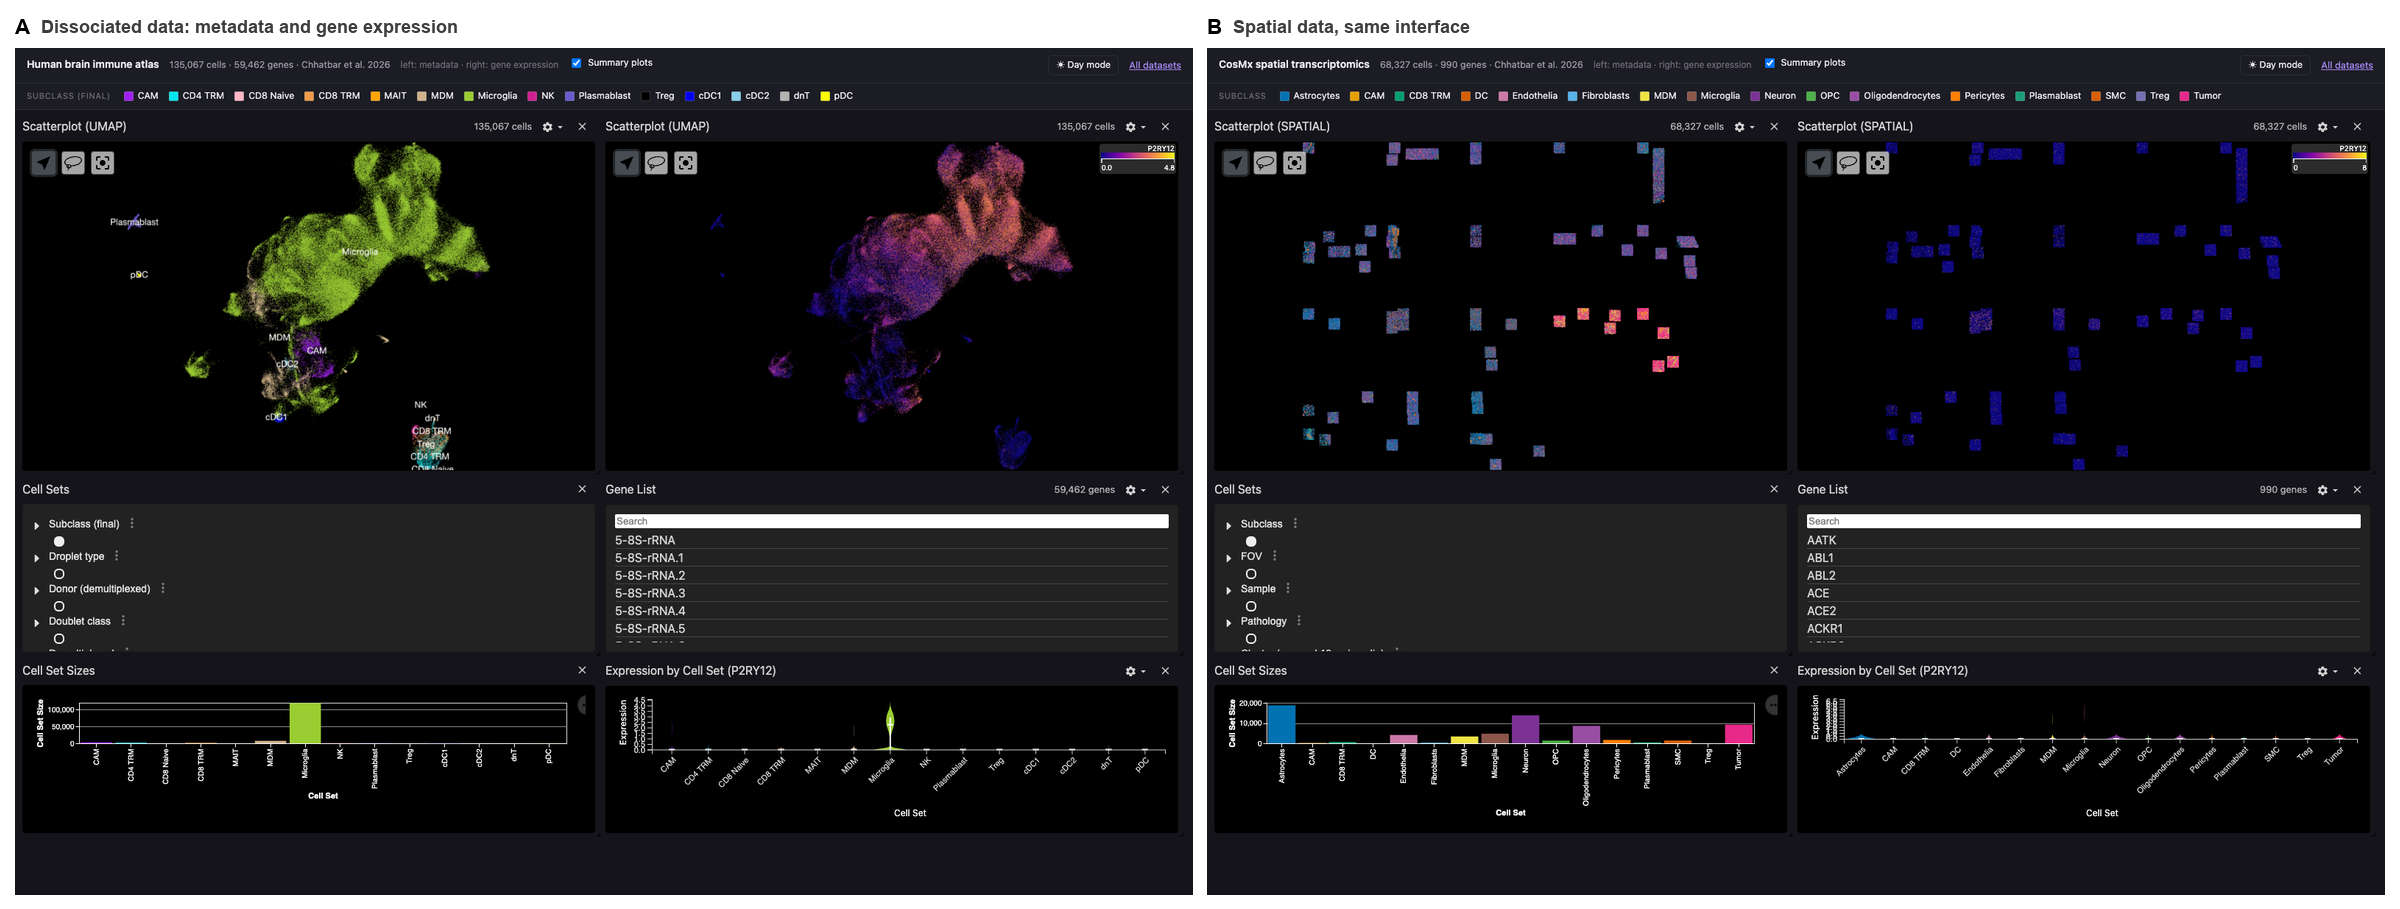
\includegraphics[width=0.72\textwidth]{figure1.png}
  \caption{The generated viewer, shown on two of the \NumDatasets{} datasets.
  (\textbf{A}) Dissociated data: two linked embeddings of a 135,067-cell human
  brain immune atlas, coloured by cell type on the left and by \textit{P2RY12}
  expression on the right, with a legend built from the authors' own palette,
  cell-set and gene pickers, and per-cell-set summary plots beneath.
  (\textbf{B}) Spatially resolved data in the same interface: Nanostring CosMx,
  with tissue coordinates supplied as an additional embedding; fields of view
  from 18 samples are laid out side by side, preserving within-sample geometry. Each dataset is a single AnnData-Zarr
  store addressed by URL, served without an application server.}
  \label{fig:viewer}
\end{figure*}

% Manuscript body. Shared by main.tex (article, two-column 86 mm) and by the
% official OUP class if you switch to it -- only the front matter differs.
%
% Headline numbers come from stats.tex, generated by
%   python scripts/make_benchmarks.py --latex
% so the prose cannot drift from Table~\ref{tab:benchmarks}.

\section{Introduction}

Making a single-cell dataset genuinely reusable is harder than depositing it.
Count matrices in GEO require the reader to rebuild an analysis before they can
look at anything; the \texttt{.rds} files that accompany many papers preserve
the authors' embeddings and annotations but demand a compatible Seurat version
\citep{hao2024seurat} and, for larger objects, tens of gigabytes of memory. In
the collection described here, one 135,067-cell object occupied 14.9~GB in
memory. A reader who wants to check whether one gene marks one cluster should
not have to pay that cost.

Interactive browsers address this, but the established options impose their own
constraints. Hosted platforms such as CZ CELLxGENE Discover
\citep{czi2025cellxgene} and the UCSC Cell Browser \citep{speir2021cellbrowser}
require datasets to be submitted and conformed to a schema, and control of the
presentation passes to the host. Self-hosted browsers need a process running per
dataset, a poor fit for a laboratory that wants a link to outlive a grant.
Vitessce \citep{keller2025vitessce} removes the server requirement by reading
Zarr stores \citep{moore2021ngff} directly in the browser, but leaves the
conversion, chunking and configuration to the user --- the step that in practice
determines whether the result is usable.

We provide that step. The pipeline is deliberately conservative: it re-runs no
clustering, integration or embedding, and preserves published annotations and
coordinates verbatim, so what a reader sees is what the paper reported.

\section{Implementation}

The pipeline runs as eight resumable stages driven by a single command-line
interface. Stages 1--3 are R, working with Seurat objects; stages 4--8 are
Python, working with AnnData \citep{virshup2024anndata} and Zarr. Every stage
writes a per-dataset log, records failures without halting the remaining
datasets, and skips work whose output already exists.

\subsection{Discovery, inventory and memory containment}

The input directory is walked for \texttt{.rds}, \texttt{.qs}, \texttt{.qs2},
\texttt{.H5Seurat} and \texttt{.RData}/\texttt{.rda} files, compressed or not,
and a stable key is derived from each path. Stage~1 records cells, features,
assays, layers, reductions and per-column metadata types, together with md5
fingerprints of barcodes, features and embeddings; these fingerprints identified
two files in our collection as the same cells re-exported under different names.

Objects in this collection reach 18.5~GB resident. Stages 1--3 therefore run
each dataset in a child R process, so that only one object is ever in memory,
the operating system reclaims it between datasets, and the parent measures the
child's true peak resident set size rather than estimating it.

\subsection{Trimming and verified conversion}

Stage~2 retains the normalised \texttt{data} layer of one assay, plottable
metadata and two-dimensional embeddings, and computes a highly-variable-gene
flag where none is present. Colour columns of the form \texttt{Subclass\_color}
are matched to the label column they determine by functional dependency --- name
matching and cardinality matching both give wrong answers on real objects ---
and are lifted into the view configuration, so the viewer reproduces the
authors' own palettes. Character columns that are really numeric are coerced
only when they parse cleanly; where coercion would silently delete values, such
as fetal ages recorded as \texttt{pcw\_14} beside numeric years, the verbatim
column is retained alongside the coerced one.

Stage~3 attempts conversion with \texttt{anndataR}, then \texttt{sceasy}, then a
direct \texttt{reticulate} writer, and accepts a writer's output only after
re-reading the file and confirming dimensions, barcode and feature names,
embedding shapes, the highly-variable flag, and 100 random expression values,
half of them forced onto non-zero entries. On our objects \texttt{sceasy} fails
this check: it writes \texttt{obsm/X\_ref.umap} where scanpy conventions
\citep{wolf2018scanpy} require \texttt{X\_ref\_umap}, and omits the
\texttt{highly\_variable} column. Without the check, the defect would have
reached the browser as a silently missing embedding.

\subsection{Chunking for single-gene queries}

Stage~4 writes the expression matrix \texttt{X} as a dense array chunked
$(n_\mathrm{cells}, k)$ along the gene axis, so that colouring an embedding by
one gene is a single chunk request rather than a scan. Vitessce's
\texttt{optimize\_adata} helper is used for \texttt{obs}, \texttt{var} and
\texttt{obsm}, but not for \texttt{X}: its densification path materialises the
entire matrix, which for $135{,}067 \times 59{,}462$ float32 values is 32~GB. We
stream \texttt{X} into the Zarr array in column blocks instead, so peak memory
is one block regardless of dataset size. The chunk width $k$ defaults to 10 and
widens for small datasets so that no chunk falls below 64~KB; at 363 cells the
default produced 1{,}940 files for 484~KB of data.

\subsection{Configuration, validation and release}

Stage~5 emits one Vitessce view configuration per dataset, with absolute URLs
derived from a single base URL so that changing host is a one-line edit.
Colours for every categorical column are written into the configuration rather
than assigned at runtime, which is what allows the interface to show a legend
guaranteed to match the plot. Stage~8 generates a static site: an index of
publications, one page per publication, and a viewer presenting two linked
embeddings --- one coloured by a metadata column, one by a gene --- with
cell-set and gene pickers and per-set summary plots (Fig.~\ref{fig:viewer}).
Datasets with spatial coordinates expose them as an additional embedding, so the
same interface serves dissociated and spatially resolved data.

Stage~6 verifies Zarr metadata, times single-gene fetches, confirms that every
path referenced by a configuration resolves, and screens \texttt{obs} for free
text, dates and identifier-shaped columns for manual review before release.
Stage~7 generates, but never executes, the object-store synchronisation
commands, bucket policy and CORS configuration.

\section{Results}

Applied to \NumDatasets{} datasets from five publications
(Table~\ref{tab:benchmarks}), the pipeline produced \StoreSize{}~GB of stores
from \SourceSize{}~GB of serialised objects, comprising \NumObjects{} objects
and \NumCells{} cells across scRNA-seq, snRNA-seq, CITE-seq, Nanostring CosMx
and Visium HD, in human and mouse. Conversion is a one-off cost of seconds to
minutes per dataset.

Because a single-gene query resolves to exactly one chunk request, the
format contributes little to query time: against a local HTTP server the median
across datasets was \MedianPfifty{}~ms, so end-user latency is dominated by
round-trip time to the object store rather than by the store layout. The
quantity that does scale with dataset size is transfer volume, which reaches
\MaxKbPerGene{}~MB per gene for the \BiggestCells{}-cell dataset, where one
chunk carries ten genes for every cell.

Correctness is enforced rather than asserted: the round-trip check rejected one
of three candidate writers on this collection. A self-test builds a synthetic
dataset, runs all eight stages and makes 19 assertions about the outputs, so the
pipeline can be exercised without access to any real data.

\section{Discussion}

The approach trades flexibility for durability. A static store cannot filter or
recompute server-side; what it offers is a resource that costs nothing to keep
running and cannot break when a server is decommissioned. Two limitations follow
from the chunking. Expression is stored densely, so a store is larger than a
sparse representation would be for very sparse data; and a fixed chunk width
means large datasets transfer more per gene than they strictly need, which
narrower chunks would reduce at the cost of more objects. The Vitessce heatmap
view is impractical at this scale, as it requires the whole filtered matrix ---
approximately 2~GB for a $135{,}000 \times 4{,}000$ selection --- so colouring
an embedding by a gene is used instead.

The pipeline preserves each dataset's own annotations, so cell-type vocabularies
differ between studies. Harmonising them to a shared ontology would make the
collection analysable rather than merely browsable, and is the natural
extension of this work.



% --- back matter ------------------------------------------------------------
\section*{Acknowledgements}
TODO.

\section*{Funding}
TODO.

\section*{Conflict of Interest}
None declared.

\bibliography{references}

\end{document}
